%%% Clinic Statement of Work Template

%%% !!! HMC STUDENTS SHOULD REMOVE THE FOLLOWING COPYRIGHT NOTICE FROM
%%% !!! FINAL SUBMISSIONS.

%%% Copyright (C) 2004-2015 Department of Mathematics, Harvey Mudd College.
%%%
%%% This file is part of the hmcclinic class document provided to
%%% HMC mathematics students.
%%%
%%% See the COPYING document, which should accompany this
%%% distribution, for information about distribution and
%%% modification of the document and its components.

%%% !!! END COPYRIGHT NOTICE.


%%% Clinic reports use the hmcclinic class, which should be located
%%% somewhere in TeX's search path.

%%% You must set a document-class option to tell the class what
%%% department your report will be for.
\documentclass[cs,proposal]{hmcclinic}
\usepackage{enumitem, graphicx, fancyhdr}

%% Supported department classes are
%%
%%    biology
%%    computer-science
%%    chemistry
%%    engineering
%%    mathematics
%%    physics

%% For your Statement of Work, use "proposal", as set above.


%%% The major difference between the Statement of Work and a midyear
%%% or final report is that the statement of work is typeset as an
%%% article, which means that the highest level of structural
%%% division available to you is \section rather than \chapter.

%%% There are also some changes in pagination styles and content
%%% that reflect the briefer nature of the proposal.  For example,
%%% in the longer reports, you use \frontmatter, \mainmatter, and
%%% \backmatter to separate some sections of the report from
%%% others.  In the statement of work, you don't need those
%%% commands, as no such division is necessary.

%%% Other packages needed by your document may be loaded here.
% \usepackage{url}              % For formatting URLs and other web or
                                % file references.

%%% Provide additional context around errors. 
\setcounter{errorcontextlines}{1000}


%%% Information about this document.

%%% I find it most useful to put identifying information about a
%%% document near the top of the preamble.  Technically, this
%%% information must precede the \maketitle command, which often
%%% appears immediately after the beginning of the document 
%%% environment.  Placing it near the top of the document makes it
%%% easier to identify the document, and keeps it out from getting
%%% mixed up with the real meat of the document.

%%% We use the same set of commands for specifying information about
%%% the people involved with the project that are used in the longer
%%% reports, so you can copy most of this information directly into
%%% your midyear and final reports.

%%% So, some questions.

%% What is the name of the company or organization sponsoring your project?
\sponsor{Proofpoint, Inc.}

%% What is the title of your report?
\title{Predicting Malicious URLs}

%% Who are the authors of the report (your team members)?  (Separate
%% names with \and.)
\author{Vidushi Ojha (Project Manager) \and James Best \and Aidan Cheng \and Kevin Herrera \and Carli Lessard}

%% What is your faculty advisor's name?  (Again, separate names with
%% \and, if necessary.)
\advisor{Elizabeth Sweedyk}

%% Liaison's name or names?
\liaison{Thomas Lynam \and Mike Morris}

%% Did you have an outside consultant help you with this project?  Put
%% their names in the \consultant command.
%\consultant{Joseph Jones}

%%% End of information section.

%%% New commands and environments.

%%% You can define your own commands and environments here.  If you
%%% have a lot of material here, you might want to consider splitting
%%% the commands and environments into a separate ``style'' file that
%%% you load with \usepackage.

\newcommand{\coolcommand}[1]{#1 is cool.} % Lets everyone know that
                                % the person or thing that you provide
                                % as the argument to the command is
                                % cool.


%%% Some theorem-like command definitions.

%%% The \newtheorem command comes from the amsthm package.  That
%%% package is *not* automatically loaded by the class file, so if
%%% you choose to use these commands, you'll need to specify the
%%% "amsthm" document-class option.

%%% Note that these definitions have changed from the version in the
%%% sample report document by dropping the ``within'' argument.  See
%%% Gratzer's _Math into LaTeX_ or the AMS-LaTeX documentation for
%%% more details.

% \newtheorem{thm}{Theorem}
% \newtheorem{Theo1}{Theorem}
% \newtheorem{Theo2}{Theorem}
% \newtheorem{Lemma}{Lemma}


%%% If you find that some words in your document are being hyphenated
%%% incorrectly, you can specify the correct hyphenation using the
%%% \hyphenation command.  Note that words are separated by
%%% whitespace, as shown below.

\hyphenation{ap-pen-dix wer-ther-i-an}

\pagestyle{fancy}
\fancyhf{}
\fancyhead[LO,RE]{\textbf \thepage}

%%% The start of the document!

%% The document environment is the main environment in any LaTeX
%% document.  It contains other environments, as well as your text.

\begin{document}

%%% In a longer document (such as your midterm and final reports),
%%% you would have separate \frontmatter, \mainmatter, and
%%% \backmatter commands to define some large chunks of your
%%% document.  For the Statement of Work, which is a short document,
%%% we don't need these commands.

%%% Your Statement of Work begins with a title page.  The title page
%%% is formatted by commands in the document class file, so you
%%% don't need to worry about what it looks like -- just putting the
%%% \maketitle command in your document (and filling in the necessary
%%% information for the identification commands above) is enough.
\maketitle

\tableofcontents

%%% In a longer document or an article being submitted to a journal
%%% or conference, you would probably have an abstract that
%%% summarized the purpose of the document.  We don't need that for
%%% a Statement of Work.

%%% Similarly, in longer documents you would probably have commands
%%% to include a table of contents and lists of figures or tables.
%%% For a short document such as the Statement of Work, we don't
%%% need these commands.


%%% Content.

%%% For smaller documents---especially those you're writing by
%%% yourself---you might write your entire report using a single LaTeX
%%% source file.  For larger documents, we recommend that you split
%%% the source file into several separate, smaller files.  The smaller
%%% files are ``included'' into your main, or ``master'' document
%%% using \include commands.  See the template file for the Clinic
%%% reports for more details on how to split a LaTeX project into
%%% smaller files.


%%% The body of your Statement of Work should appear here.  See
%%% Chapter 4 in _The Mathematics Clinic in Brief: A Handbook_ for
%%% more details on what you should include in a Statement of Work.

\newpage

%%%

\section{Project Motivation}

Proofpoint is a cybersecurity company that provides security and data protection solutions to other companies. Amongst their many products, they provide an inbound email URL screening service that scans URLs embedded in clients' emails, and determines whether or not they lead to sites containing malware.

Determining the maliciousness of URLs is a critical component of Proofpoint's security suite because of the ease with which malware can affect clients' machines. Malware can covertly install itself when a user clicks on a URL, and compromise personal and sensitive information without the victim knowing it. Indeed, attackers can send emails containing these malicious URLs from seemingly benign sources, like someone in the victim's address book, making such emails hard to detect for the client. Thus, Proofpoint would like to to block URLs before they even get clicked.

Proofpoint's solution currently redirects every URL embedded in an email through their servers, where they employ a filter to distinguish between URLs that should and should not be blocked. Their current filtration technique has approximately 70\% accuracy in determining whether a URL is malicious. This method checks how many times the URL appears in a certain time period and context, and how many domains it goes through.\footnote{These heuristics are useful because they provide characteristics common to malicious URLs. Many will be sent through multiple domains to try to hide where they came from, and they will be sent multiple times to try to get through to the client.} If a URL reaches a certain threshold with regards to these two test metrics, it will be sent to Proofpoint's \textit{sandboxing environment} for further testing. Sandboxing, the practice of opening a URL on a virtual machine and simulating its effects, is currently the most accurate method of determining whether a URL is malicious. If the sandbox becomes infected with malware, Proofpoint will block that URL in the future.

However, sandboxing is slow, which makes it expensive in both time and money. Given the billions of emails Proofpoint's security suite sees every day, it is unfeasible to sandbox every single one. It would therefore be useful to have a more effective way of determining which URLs are malicious, as this would significantly reduce the number of URLs that have to go through the expensive sandboxing process.

Although their current method of predicting malicious URLs is relatively effective, there is much room for improvement. Proofpoint is interested in improving the number of URLs blocked overall, but also the number of URLs blocked before the client has a chance to click on them. Our team believes that methods of machine learning are well suited for this problem: given the vast amounts of data, classification and pattern matching are exactly the kinds of solutions needed for this problem. Our hypothesis is that there are common characteristics shared by malicious URLs, and indeed, others before us have investigated such characteristics (see section \ref{feature-selection}). An effective learning technique could determine these characteristics and use them as facets of a learning model. For this reason, we plan on employing a number of different machine learning techniques to the malicious URL detection problem.

%%%

\section{Problem Statement}

Proofpoint processes billions of URLs a day to determine if they are malicious. However, their sandboxing method is much too expensive a process for it to be attempted for every URL they see. Thus, there is a need for better predictive model that reduces the number of expensive sandbox tests that must be performed. This system should learn from existing metadata about URLs. The ideal solution for this problem would be able to learn from its predictions. For example, if it predicts a URL to be malicious, and that URL is deemed safe by the sandboxing environment, the predictor should refine its model to account for this data. The problem, then, is to construct a model with these characteristics that can make these predictions for the vast number of URLs being processed by Proofpoint on a daily basis.

%%%

\section{Goals}

Over the course of this academic year, our team intends to design and implement a system that uses machine learning to detect malicious URLs before they are clicked. The primary aim of this systems is to block these URLs before Proofpoint's clients view them, thereby avoiding any opportunity for the URL to be clicked. However, while the primary goal is to block URLs before they are clicked, there are three metrics total that will be measured in order to evaluate the success of our model. These are:

\begin{itemize} \itemsep0em
\item The proportion of malicious URLs tagged as malicious before they are clicked
\item The proportion of malicious URLs tagged as malicious total
\item The proportion of malicious URLs submitted to the sandbox for additional analysis
\end{itemize}

We are aiming to improve upon the current proportion of URLs blocked before clicking, which is currently at around 70\%. Although we have no precise numbers to outperform with regards to the other two metrics, our aim is to accurately block as many URLs as possible while minimizing inaccurate predictions.

The system we aim to build must have the following features:

\begin{enumerate} \itemsep0em
\item For any given input URL that is given to it, the system returns a score between 0 and 1, where the score indicates the probability of the URL being malicious.
\item Using the above score, each sample will be classified as either dangerous or not, based on some cutoff. For instance, if we decide on a cutoff of 0.7, then anything with a score of 0.7 or above will be considered dangerous.
\item Our model will explain how the score was assigned, for instance by pointing to characteristics of the URL that make it more likely that it is malicious.
\end{enumerate}

%%%

\section{Classifier Types}

The following are summaries of the classifiers our team will investigate over the course of this project.

\subsection{Naive Bayes}

The first approach we want to apply to this problem is a Naive Bayes classifier. This classifier relies on a \textit{Bayes' net} to understand the relationship between different characteristics of a data sample, called features. To construct a Bayes' net, we will construct a set of features that we believe are related to a URL being malicious. These features are typically binary: for instance, ``is the URL above 20 characters in length or not?'' could be a feature. The Bayes' net is then a directed acyclic graph, where nodes represent features, such as the above example of URL length and, importantly, the feature of being malicious or not. The directed edges between features encode the idea of conditional dependence. This can be thought of as causality: in putting an edge between ``is the length over 20 characters?'' and ``is this URL malicious?'', the Bayes' net is signifying that there is some type of causal link between these features. A Bayes' net where we assume that all the variables are independent is called naive.

To use such a Bayes' net as a classifier, we use probability distributions to describe the likelihood of any URL sample possessing the features in the net. We can then use the joint probability distribution of all the variables, as well as formulae for conditional probability, to compute the probability that a particular sample possesses the feature ``is this URL malicious?''. 

Note that the other features in the net must have established probability distributions in order for this to be possible. We propose that these probabilities be computed by taking the frequency with which they appear in the training data set. This, along with the Bayes' net we will construct, provides us with all of the information needed to compute a probability regarding the URL's nature.

There are two important advantages to this approach. First of all, our established goal was to provide a continuous spectrum along which we could rank URLs (for instance, percent likelihood of being malicious), rather than a discrete classification (``malicious'' or ``not malicious''). By using probabilities, we could find that a URL is anywhere between 0 and 1 in its maliciousness ranking. Second, we believe that by using features and a Bayes' net, we should be able to reverse engineer a given URL's ranking to find which features contributed to its score. This means that if a URL is marked as malicious, it is straightforward to find why our model classified it as such.

\subsection{Support Vector Machines}

Another approach we will consider in our solution is using a support vector machine (SVM). A support vector machine is a supervised learning model that classifies data into one of two categories. An SVM maps data points into an $n$-dimensional space, where $n$ is the number of features being considered. The SVM then constructs a hyperplane that divides the points (which represent the objects being classified) into two parts, such that the distance between the plane and the closest point on either side is maximized. When new data is given to the SVM, it predicts which category the data belongs in based upon which side of the plane it falls on.

There is existing research in the effectiveness of SVMs in spam filtering (Sculley and Wachman). One problem with using SVMs with this type of problem is the increased training time as the size of the data set increases. In the study by Sculley and Wachman, an approach that was successful in combatting this problem is using a relaxed online SVM to achieve an approximate solution. A relaxed online SVM updates its model less frequently than an offline SVM, and it uses a sliding window over the data to ensure that the same amount of learning data is used in each update. This ensures that the training will take roughly the same amount of time each iteration. The results of this study showed that relaxed online SVMs performed nearly as well as offline SVMs that learned from all the data (Sculley and Wachman, 5).

We will investigate how beneficial using an SVM would be for our problem. Since it has proven to be effective in other text recognition problems such as spam-filtering, we believe that using an SVM could produce promising results for our classification system. In the process of implementing an SVM, we will explore open source tools and libraries that are available to us. Using an open source library can help us determine if an SVM is a valid approach to solving our problem without having the overhead of implementing our own SVM. 

\subsection{Clustering}

Another approach we will consider when we are creating or improving on our classifier is the use of cluster analysis. Cluster analysis can be simply thought of as the task of grouping up data objects into partitions or ``clusters'' such that data objects in one cluster are more similar to one another than those data objects that are in a different cluster.

The way in which these objects are clustered can vary depending on which aspect of the data is more heavily weighed as a defining characteristic of the group. There are many algorithms that can help determine which specific features of the URLs to cluster by, and so it falls upon the team to produce the algorithms that we will be using for our clustering. There are various approaches to clustering algorithms that we may take, which include: connectivity-based clustering, centroid-based clustering, distribution-based clustering, and density-based clustering. 

Furthermore, we will have to evaluate the results of our clustering. We may do so through internal or external evaluation. The former method uses the data that was clustered itself to evaluate the results while the latter uses data not used in clustering. It is also important to note that clustering is an iterative process that will need to undergo various trial and error phases in order to learn the aspects that make a good cluster.

We will investigate how we can combine cluster analysis with SVMs in order to avoid having to update the SVM model constantly, which takes a significant amount of time. Instead we only use specific clusters from our cluster analysis to update the SVMs.

%%%

\section{Feature Selection} \label{feature-selection}

For all of the classifiers discussed above, feature selection is crucial. Choosing features that serve as good indicators of positive or negative results is necessary for accurate classification. Recall that features are characteristics of the data sample being analyzed, in our case a URL embedded in an email. One example would be the number of periods in a URL.

Existing research using lexical and WHOIS features to detect malicious URLs has been quite successful, with a 90-95\% detection rate (Ma et al., 1). Lexical features are the textual properties of the URL itself, and WHOIS data gives the registration date/user of the given domain. But it should be noted that they did not consider URL page content or the type of email the URL is embedded in; they ignored such contextual information altogether.

There are a number of reasons not to consider context or page content, and concentrate on the URL itself. To download a page's content every time is expensive and slow, and does not result in a lightweight model. In addition, taking URL context into account restricts the model from being applied to contexts outside of those that it was trained on. It would be best to have a model that is flexible enough to be applied to any context (for instance, email, games, chat, calendars, etc.). 

It is also important to consider how many features to use. In the study by Ma et al., it was found that models with more features typically perform better than models with fewer features. They found that a feature set with 4 features attained a 10.12\% error rate, while a feature set with 3,967 features was able to gain a 3.22\% error rate (Ma et al., 5). Thus, more features do seem to lead to better results. However, existing research seems to suggest that there are diminishing returns for every feature we put in after a certain point.

Since we are not given the WHOIS data in the URL dataset given to us by Proofpoint, we will have to construct features of our own that perform just as well. We would like to investigate whether it would be possible to lookup WHOIS features for URLs our model is less certain about, but this will depend on whether Proofpoint is interested in allocating computing power for such lookups.

For the purposes of our project, it seems most efficient to begin with a small number of features first. Our aim is to figure out which ones are best at differentiating malicious and safe URLs, and in later iterations considering raising the number of features.

%%%

\section{Architecture}

The general architecture of our system is laid out in Figure \ref{architecture-fig}.

\begin{figure}[ht]
  \centering
    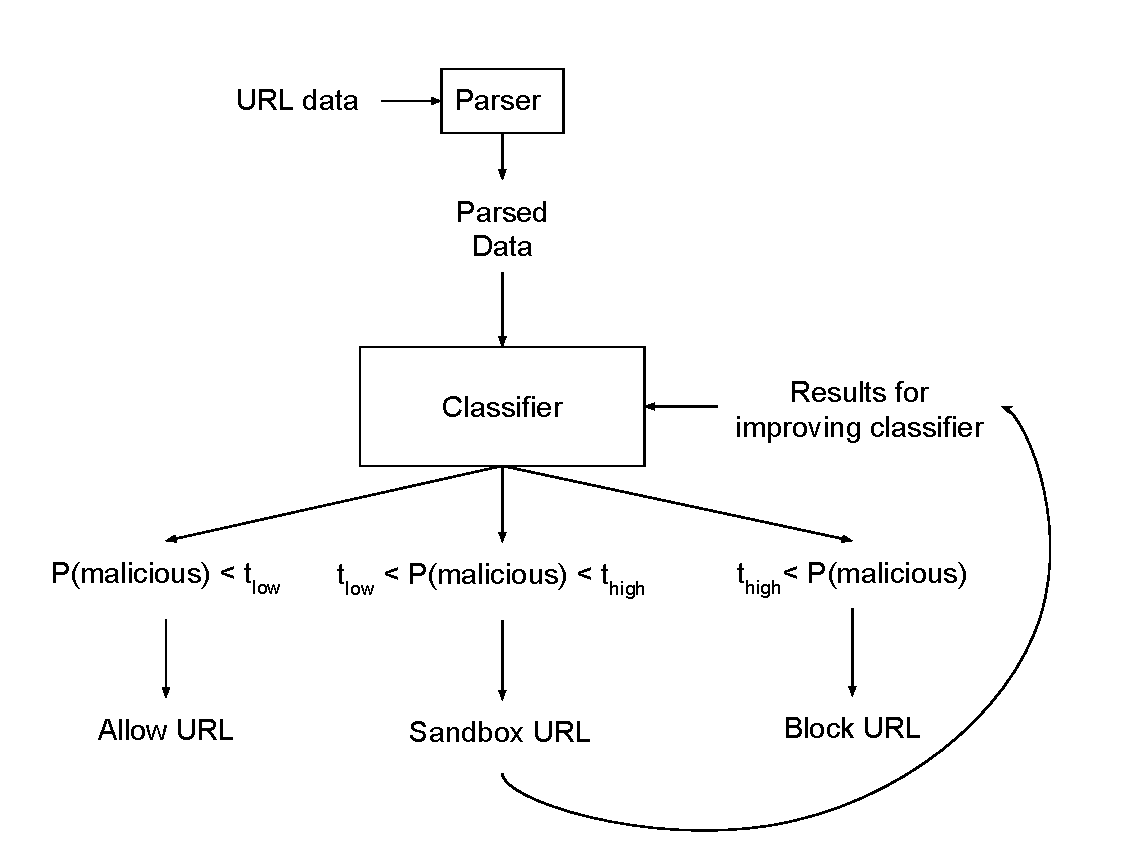
\includegraphics[scale=0.75]{architecture_diagram}
  \caption{General architecture breakdown}
  \label{architecture-fig}
\end{figure}

We begin by employing a data parser to go from the raw samples we are given to JSON objects representing the URLs and their associated metadata. The parsed data will be fed into a classifier which the system will then use to determine a probability of the URL being malicious. The result of the classifier, a probability value between 0 and 1, will then be used to evaluate the next step.

If the probability of the URL being malicious is greater than some threshold value, $t_{\text{high}}$, then it will be immediately blocked. If the probability is less than $t_{\text{high}}$, but larger than some lower threshold, $t_{\text{low}}$, then it will be sent to the Proofpoint sandbox environment where the sandbox will evaluate the validity of the classifiers decision. Finally, if the probability is less than $t_{\text{low}}$, then it will be allowed through without further analysis.

For the data objects sent to it, the sandbox will provide some results, indicating whether our classifier was accurate or not. These results will be fed back into our classifier to improve its accuracy. The algorithm will therefore be able to improve upon its detection methods and then make use of those improvements by updating the classifier with new features to detect when determining maliciousness.

We will modify the above procedure as necessary for different environments (described below) as we come closer to deploying our system.

%%%

\section{Deployment Strategy}

For this project, we plan to employ an agile approach where, every few weeks, we deliver a new or improved system and build upon our existing software after obtaining feedback on it. Thus, the process of our deployment strategy will follow these three stages:

\begin{enumerate} \itemsep0em
\item Construct a model that works in our local environment and continuously improve upon it
\item Have our system work in Proofpoint?s lab environment and acquire feedback
\item Move the system to production for additional performance evaluation
\end{enumerate}

Given that we plan to produce several versions of our software, we plan to work through several iterations of the strategy laid out above. Each version of our software will proceed through these stages with the results feeding back into previous levels in order to continuously improve on our existing systems. 

%%%

\section{Schedule}

In this section, we give an overview of schedule we plan to follow and describe the various deliverables we plan to have, as well as the tasks we intend to undertake in order to produce those deliverables. These deliverables fall under a series of phases that constitute a schedule for our project to follow.

\subsection{Phases Overview}

Phase 1:
\begin{itemize} \itemsep0em
\item Two initial versions of our classifier using Naive Bayes and SVMs
\end{itemize}

\noindent Phase 2:
\begin{itemize} \itemsep0em
\item Software that surpasses the 70\% accuracy threshold, using some combination of the Phase 1 classifiers
\item Additional classifiers employing other approaches, if necessary
\item Mid-year report
\end{itemize}

\noindent Phase 3:
\begin{itemize} \itemsep0em
\item Improved software that surpasses previous milestones in accuracy
\end{itemize}

\noindent Phase 4:
\begin{itemize} \itemsep0em
\item Final version of software
\item Final report
\item Project poster
\end{itemize}

\subsection{Workflow and Deliverables}

In order to follow through with our agile deployment strategy, we have set up a series of tasks that will allow us to quickly iterate through different versions of our system. In each iteration of our software development the tasks are to design, build, test, and assess a new classifier, or a new version of a previous classifier. We expect to have at least two subteams working on unique approaches to our software at all times.

To this end, we will begin Phase 1 by working on two approaches to our classifier, Naive Bayes and SVMs. Within the month of October we expect to have our first deliverable: a basic URL classifier that, when given a URL and meta-data about the URL, predicts the probability of the URL being malicious or not. It is important that our code is well-documented because it may be used or altered by other people in the future; therefore, we will have documentation within the classifier that will assist readers in understanding our design.

Once our two initial programs are completed, we plan to move into the next phase of our initial iteration where the team will focus their efforts into improving the initial software and possibly reiterate through Phase 1 with a new version of a classifier that uses a different approach. We may, at this point, pick one classifier to focus our efforts on. We hope to be working in the Proofpoint lab environment and making use of the sandboxing environment in order to improve our classifier?s detection rate.

The second deliverable that we expect to have at the end of this phase is a working classifier with a malicious URL detection rate of above 70\%. During this time we will also be working on our third deliverable for this phase, a mid-year report. This is an update where we describe our progress on the project, design decisions that we have made, and a detailed description of what we will do in the second half of the year.

Our third phase mainly consists of the team surpassing previous milestones in accurate detection rate. We expect that by this point we will be focusing our efforts on mainly building upon existing systems rather than creating new ones. New features and machine learning techniques will be incorporated into the current system in an attempt to improve it. We hope to be at this point of our project by the start of the spring semester.

The final phase of our project's schedule includes various deliverables that we will be focusing on in order to conclude our project. The main deliverable of this phase is the final version of our software which will be the cumulative product of all our work during the year. We expect to have a system with a high detection rate and appropriate features by this point. We will also have the corresponding documentation to go along with our system. The second deliverable for the final phase is a  final report that summarizes the results of our project. This report will give an overview of the problem, a description of what we did over the course of the year, any results we obtained from our project, and recommendations for future work. The final deliverable is a poster summarizing our project and the progress we made over the course of the year.

%%%

\section{Tools}

In order to manage the code we write and to have version control, we will be using Git and GitHub to store our repository privately.

Additionally, we will use our team's Trac web page to manage our documents and other organizational items we use over the course of the year.

We intend to primarily use Python for its native JSON support and the many Python machine learning libraries available open source. In addition, prior research has suggested use of MATLAB for classification purposes, making it a viable alternative. For instance, MATLAB has many useful built-in functions that can help us get started as quickly as possible, such as the statistics and machine learning toolbox, which already has a Naive Bayes classifier built into it.

%%%

\section{References}

\hangindent=2em
\hangafter=1
Ma, Justin, Lawrence K. Saul, Stefan Savage, and Geoffrey M. Voelker. ``Beyond Blacklists.'' \textit{15th ACM SIGKDD International Conference on Knowledge Discovery and Data Mining}, 2009, New York, USA. Unpublished conference paper. UCSD Library, 2016. Web.

\hangindent=2em
\hangafter=1
\noindent Sculley, D., and Gabriel Wachman M. ``Relaxed Online SVMs in the TREC Spam Filtering Track.'' \textit{16th Text Retrieval Conference}, 2007, Maryland, USA. Unpublished conference paper. Tufts University Library, 2016. Web.

\newpage



%%% Appendices.

%%% For your Statement of Work, you probably won't have any
%%% appendices, but you could include some if you really needed to.

%%% The appendices are delineated with the \appendix command.
%%% Individual appendices are begun with the standard \chapter or
%%% \section commands.  In our example, we'll \include them just as we
%%% did other chapters.

%%% Even in a relatively short document such as your statement of
%%% work, you might need to have appendices.  If so, uncomment
%%% the \appendix command and add them below (remember, the
%%% top-level structural command in this format is section).

% \appendix

%%% Bibliography.

%%% BibTeX is the tool to use for citations and layout of your
%%% bibliography.  Instead of having to type ``[5]'' or ``(Jones,
%%% 1968)'' (and keep track of which citation is which and renumber
%%% them as you add more references to your bibilography), you use
%%% special commands that allow BibTeX and LaTeX to automatically put
%%% the correct information in the right place.

%%% Section 5.6 in _The Mathematics Clinic in Brief: A Handbook_,
%%% talks about using BibTeX to format your bibliography and
%%% citations.

%%% Depending on your field, it may or may not be appropriate to list
%%% references for which you haven't included specific citations.  If
%%% your field sanctions such practices, or if you just want to get an
%%% idea of what you have in your bibliography file, you can include
%%% everything with the \nocite{*} command.
\nocite{*} 


%%% The appearance of your bibliography and citations in your text are
%%% defined by a combination of any bibliography-related LaTeX
%%% packages (such as natbib, harvard, or chicago) and the particular
%%% bibliography style file that you load with the \bibliographystyle
%%% command.  Bibliography-style files end in .bst; you can find them
%%% by searching your file system using whatever tools you have for
%%% doing searches.  (On most modern Unices, ``locate .bst'' will give
%%% you an idea of what's available.)

\bibliographystyle{hmcmath}

%%% The particular bibliography data file or files that you want to
%%% use are specified with the \bibliography file.  Multiple files are
%%% separated by commas.

%%% You might want to use multiple bibliography (or ``bib'') files if
%%% you had a master bib file containing references you use again and
%%% again, and another containing only records for references for a
%%% particular project.

%%% Many people create a single, large bib file that they use for
%%% everything they write.  That approach requires you to \cite every
%%% reference that you want to use in your document -- using
%%% \nocite{*} with a huge bibliography database will give you a large
%%% bibliography containing many references you haven't consulted for
%%% your particular document!

\bibliography{sample}


%%% Glossary or Index.

%%% Having a glossary or index in a statement of work is overkill.
%%% Just define your terms in the text and you'll be fine.

\end{document}
